\documentclass[11pt]{article}
\usepackage{array}
\usepackage{tabularx}
\usepackage{graphicx}
\usepackage{caption}

\title{
	\textbf{Computer Vision AI - Final Project Report}
}

\author{Tobias Stahl \\ 10528199 \and Ioannis-Giounous Aivalis \\ 10524851}

\usepackage{amsmath}
\begin{document}

\maketitle

\section{Introduction}
In this report we will introduce the methods used in order to achieve  the goal of animal detection from images captured by drones. More specifically the task of this assignment has been the automatic detection of rhinos from images captured by drones in the fields of South Africa.
bla \cite{Sochman07learninga}

\section{Motivation}
Recently the horn of the rhino has been claimed to be a form of alternative medicine and a status symbol amongst some countries of Asia. This has lead to intense hunt of the animal by illegal poachers in order to extract the horn and illegally sell it to rich people who have the ability to pay for it in those countries.\\
The majority of the population of the rhino inhibit the Kruger National Park which covers an area of almost 20 thousand square kilometers. It can be now easily seen that protecting the animal within the confounds of the park by human rangers is a task that cannot be achieved without the help of some automated mechanism. In that direction, our methods come to serve as a complementary resource to the ranger who will receive spatio temporal information from the drone about the location of the animals or poachers.\\
For the realisation of this project we worked with a dutch team who is occupied on this task, namely the Dutch UAS (Unmanned Aerial Solutions).

\section{Requirements}
The Dutch UAS team already uses drones with high end cameras and network capabilities. Our task however mostly concentrates on speeding up the detection time by preserving an accuracy standard. Ideally we would like to minimize the true negative rate to a minimum since the detection of the rhinos is the important task at hand. 

\section{Related Work}
Object detection has been a traditional computer vision task for many years, many methods have been implemented to achieve this task through the years, each of which comes with their own set of advantages and disadvatages. Dalal et al \cite{dalal2005histograms} tackle this problem (for the human detection scheme) by using histograms of oriented gradients (HOGs) which provided one of the most influential solutions for this task at the time. A mixture of deformable part models was introduced by Felzenszwalb et al \cite{lsvm-pami}. They too made use of HOGs along with some matching algorithms for deformable part-based models. Van de Sande et al \cite{vandeSande:2011:SSS:2355573.2356474} introduce image segmentation as a form of preprocessing images to solve the detection problem and achieved a very high accuracy for the PASCAL VOC 2007 dataset. Lastly, Wang et al \cite{Wang:2013:RGO:2586117.2587017} make use of regionlets (base feature extraction regions defined proportionally to a detection window at an arbitrary resolution) organized in small groups to delineate fine grained spatial layouts inside objects. Those papers have introduced new methods for the task of object detection, they all make use of SVMs, which is aims for accuracy in the multiclass classification problem. However the task at hand is bounded by time, which means that we need to determine whether or not a given frame contains an animal as soon as possible, with accuracy not being the main concern.\\
In this direction, the paper introduced by Viola and Jones \cite{Viola01rapidobject} uses boosting for the task of real-time face detection reaching speeds up to 15 frames per second without resorting to image differencing or skin color detection. In this approach Haar-like features are used since they are really fast to compute by using only the integral image. Furthermore the boosting algorithm allows for fast decision making in comparisson to SVMs.

\section{Approach Overview}
The task of real-time object detection has been successfully tackled by Viola and Jones using adaboosting on Haar features, therefore we also implemented an Adaboost pipeline for our problem. In this section we will present this pipeline along with the improvement we introduced which is based on an adaptation of the Waldboost \cite{Matas05waldboost-} algorithm for our needs.

\subsection{Adaboost baseline}
Adaboost short for Adaptive Boosting is a machine learning algorithm introduced by Freund et al \cite{Freund99ashort}. Boosting is an efficient method of learning by avoiding overfitting to training data. It defines a classifier using a weighted additive model which consists of many weak learners. The output of the classifier is the weighted sum of those weak learners. The individual learners themselves are weak in the sense that their accuracy needs be slightly better than random (i.e. their error rate needs to be slightly less than 0.5).\\
Unlike neural networks and SVMs, the AdaBoost training process selects only those features known to improve the predictive power of the model, reducing dimensionality and potentially improving execution time as irrelevant features do not need to be computed. The final strong classifier after training looks like this:
\[ 
F(x) = \sum_{t=1}^{T} \alpha_t f_t(x)
\]
In this equation: $T$ is a parameter of the classifier and it denotes the number of weak learners the classifier consists of, $\alpha_t$ is the weight of the weak learner and $f_t$ is the response of the weak classifier $t$ for the given sample $x$.\\
As per protocol in the boosting scenario all the patches are initially equally weighted. After each training cycle, misclassified patches are assigned a higher weight so as to be taken "more into consideration" by the next iterations and those who were already correctly classified are assigned a smaller weight. Figure \ref{reweighting} illustrates the process of sample reweighting in two subsequent iterations. In this Figure the green line denotes the threshold of the weak classifier upon which the classification decision is made. The radius of the misclassified samples increases according to their weight increase in the second iteration. 

\begin{tabular}{ll}
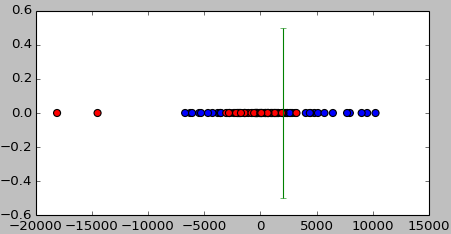
\includegraphics[scale=0.380]{res/left.png}
& 
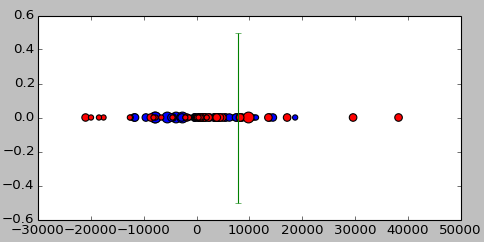
\includegraphics[scale=0.370]{res/right.jpg}
\\
\label{reweighting}
\end{tabular}
\captionof{table}{Visualization of the sample reweighting} 

\subsection{Waldboost}
On the foundations set by Adaboost, Waldboost \cite{Matas05waldboost-} introduces the possibility of reducing the classification time even further, by picking a small ammount of the classifiers that would be used for Adaboosting. Unlike Adaboost, each discrete classifier has the capability of coming to a final decision about a given patch under specific circumstances. That means that the classification time significantly reduces since it does not necessarily require use of all the weak learners.\\
The learning process is implemented similarly to Adaboost, in each iteration, the weak learner minimizing the error for a given training set is appended to the classifier. Unlike Adaboost a random subset of the training set is used in each iteration.\\
In order to determine the circumstances under which a weak learner is able to reach a verdict about a given patch two thresholds for the returned values need to be determined, above and below which, the weak learner at hand is decisive. These thresholds are the $\theta_a$ and $\theta_b$ which are specific for each given layer of the classifier. In order to determine those thresholds we call upon Wald's Sequential Probability Ratio Test based on Wald's sequential analysis \cite{Wald:1947}.\\
The two thresholds specifying if a sample can be classified in a certain iteration of the classification, are found by comparing the likelihood ratio of the samples with fixed thresholds $A$ and $B$, which are computed with the input parameters $\alpha$ and $\beta$ determining the false positive and false negative tolerance rate of the classifier. The threshold search on the basis of the likelihood ratio is visualized in Figure \ref{threshold}.\\
As can be seen on the left Figure, the outputs of the classifier are split per true label. The $\theta_a$ search process goes as follows: we generate the likelihood ratio (right plot) and we look for the first datapoint which satisfies the condition $R(x) > A$ where $A = \frac{1-\beta}{\alpha}$. Similar process from right to left takes place for finding the $\theta_b$ threshold. In the next step of the algorithm, all samples which can already be classified are removed from the sample pool and the focus shifts on those which cannot be classified so far


\begin{tabular}{ll}
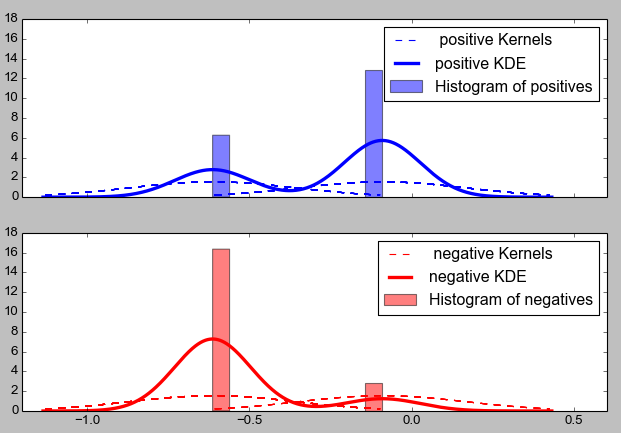
\includegraphics[scale=0.270]{res/links.png}
& 
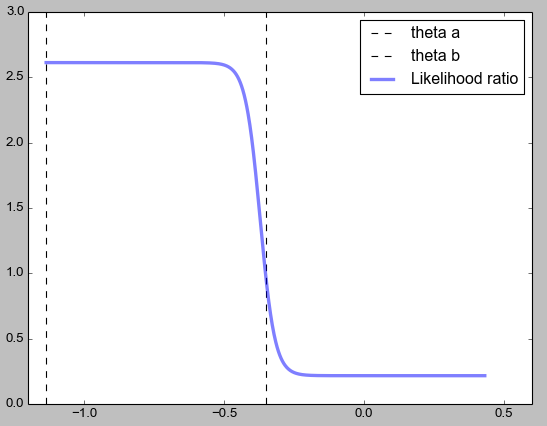
\includegraphics[scale=0.275]{res/rechts.png}
\\
\label{threshold}
\end{tabular}
\captionof{table}{Visualization of the threshold search} 

\subsection{Haar-like Features}
Since our objective is to minimize the decision time of the classification, our feature set consists of Haar-like features, according to the Viola and Jones approach. This might not be the best feature set for the detection of an animal, but since it is an easy to implement and fast feature it is sufficient for our purpose.\\
A Haar-like feature considers adjacent rectangular regions at a specific location in a detection window, sums up the pixel intensities in each region and calculates the difference between these sums. Figure \ref{haar_img} shows the 5 feature types used. With the use of integral images, a Haar-like feature of a single rectangle can be computed with as much as only three summations.\\


\begin{figure}[htp]
\centering
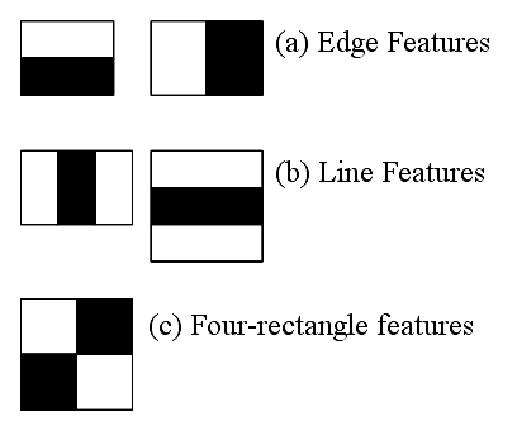
\includegraphics[scale=0.380]{res/haar.JPG}
\caption{Haar-like features used}
\label{haar_img}
\end{figure}

\section{Dataset}
Since there is no publicly available annotated data set of rhinos we know of, the Verschoor Aerial Cow Dataset \footnote{https://github.com/camielv/wildlife-monitoring/tree/master/dataset} was used, due to the similar shape of a cow and a rhino. In order to use this classifier for the rhino detection in Kruger national park, the classifier has to be re-trained with a data set consisting actual rhinos.\\
The data set consists of two videos, each containing approximately 5000 frames each. The negative samples are extracted from the background, therefore we have unlimited negative samples.

\section{Implementation}
In this section we explain some of the characteristics of our implementation.
\subsection{Weak Learner}
The weak learner is a decision stump with the threshold minimizing the classification error of the weighted patches. Initially our own method was tested to make the threshold evaluation, however in order to speedup the threshold search the scikit-learn\footnote{http://scikit-learn.org/} \texttt{DecisionTreeClassifier} was used.
\subsection{Image Preprocessing}
In order to obtain a unique size of feature sets per image patch, each patch needed to be downsampled to 24x24, which results in 162336 Haar-like features per patch similarly to the Viola and Jones implementation. Due to speeding benefit and the insignificance of the smallest Haar-like features we subsampled only Haar-like features with a size of at least 6 pixels, which reduced the feature set to 86406 per image patch.

\section{Results}
In this section we will sum up the results we obtained from running the detector that occured from using our classifier. For this detector we made use of the sliding window approach with a vertical and horizontal pixel skip rate of 6 pixels since speed is of the essense.

\subsection{Best Features}
The best features are the ones who are picked for minimizing the error. Those are contained in the top performing weak learners. For simplicity reasons and due to the fact that we used one hundred layers or more for our experiments we illustrate the top four of those in Table \ref{best_features}. In the separate figures we see the exact picel posisions which they occupy in the patches. It seems like those features capture the variation between the animal and the background since they are located on the edge of the cows.

\begin{tabular}{llll}
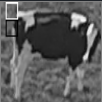
\includegraphics[scale=0.75]{res/f1.png}
& 
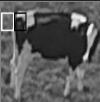
\includegraphics[scale=0.75]{res/f2.png}
&
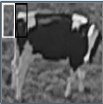
\includegraphics[scale=0.75]{res/f3.png}
& 
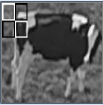
\includegraphics[scale=0.75]{res/f4.png}
\\
\\
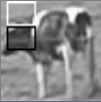
\includegraphics[scale=0.75]{res/f5.png}
& 
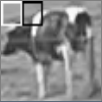
\includegraphics[scale=0.75]{res/f6.png}
&
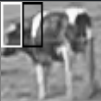
\includegraphics[scale=0.75]{res/f7.png}
& 
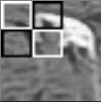
\includegraphics[scale=0.75]{res/f8.png}
\\
\label{best_features}
\end{tabular}
\captionof{table}{The four best features as chosen by the strong classifier} 

\subsection{Accuracy}
In calculating the accuracy of our detector we made a split of 750 training samples over 250 validation samples. The numbers contained in Table \ref{accuracy} indicate the errors we obtained for two settings of the classifier. The difference lies in the number of layers the strong classifier consists of.\\
\begin{center}
\begin{tabular}{l|c}
	Method type          & \textbf{Error} \\
	\hline
	300 Layers, Discrete & 0.052 \\
	100 Layers, Real     & 0.048 \\
\end{tabular}
\label{accuracy}
\end{center}
It seems like 300 layers are too many for our data set since the classifier is overfitting in that case increasing the error rate. However in both setups we achieve a very satisfactory error rate of less than 10\%.

\subsection{Time}
The initial time constraint was to achieve timing less than two seconds per frame since the drone feeds pictures every two seconds. Unfortunatelly we were not able to break this barrier since classification of images takes well over 8 seconds per picture on average. Due to time constraints we were not able to emphasise on this area, however we are confident that the timing could be improved if more effort is put into it.\\
Changing the programming environment from a \texttt{Python} implementation to \texttt{C/C++} would most likely greatly improve this area.

\section{Conclusion}
For this task we have familiarized ourselves with state-of-the-art machine learning algorithms such as Adaboost and Waldboost, we had to implement both and we gained a lot of insight in the area of computer vision and object detection algorithms. We have implemented an effitient codebase which is made available to be extended for future work and we are hopefull our implementation will be used for the cause of helping the rangers in South Africa to protect an endangered species.  

\section{Future Work}
For tackling a real world problem like the one at hand plenty of extentions have been taken into consideration. First, we think that the training time needed to extract more Haar features compared to the accuracy return of this process will be insignificant. Therefore we would consider using more than five Haar feature types. The effects of this process have been analyzed by Lienhart et al \cite{Lienhart02anextended} and show that such an approach is indeed benefitial for this cause. Another aspect that 5could enhance the performance of the detector would be not isolating the detection task, instead using some kind of tracking in order to improve the detection rates. Tracking would provide limit false detections and perhaps enable for animal counting, a task which is already under implementation. Lastly, the drone is still under construction, however when the final form of it is determined, information indicating the altitude as well as the angle of the camera could help limit the search space for the sliding window approach of the detector, since the drone flies at variant heights. 


\section{Acknowledgement}

\bibliography{biblio}

\end{document}